\documentclass[12pt]{article}
\usepackage[affil-it]{authblk}
\usepackage{polyglossia}
\usepackage[a4paper,hmargin=3.4cm]{geometry}
\usepackage{mathtools, amssymb, amsfonts}
\usepackage{amsthm}
\usepackage{fontspec}
\usepackage{titling}
\usepackage{float}
\usepackage{multicol}
\usepackage{listings}
\usepackage{graphicx}
\usepackage{xcolor}
\usepackage{mdframed}
\usepackage{titling}
\usepackage{tikz}
\usepackage{listings}
\usepackage[hidelinks]{hyperref}
\usepackage{caption,subcaption}
\usepackage{tikz}
\usepackage[locale = FR, exponent-product = \cdot, inter-unit-product = .]{siunitx}
\usetikzlibrary{arrows,shapes,calc,angles,decorations.markings,patterns,decorations.pathmorphing}
\usepackage[shortlabels]{enumitem}
\usepackage{comment}

\setdefaultlanguage{french}
\frenchspacing

\newcommand{\RR}{\mathbb R}
\newcommand{\CC}{\mathbb C}
\newcommand{\QQ}{\mathbb Q}
\newcommand{\ZZ}{\mathbb Z}
\newcommand{\NN}{\mathbb N}
\newcommand{\KK}{\mathbb K}
\newcommand{\FF}{\mathbb F}
\newcommand{\LL}{\mathbb L}
\newcommand{\PP}{\mathbb P}
\newcommand{\EE}{\mathbb E}
\newcommand{\VV}{\mathbb V}
\renewcommand{\epsilon}{\varepsilon}

%%%
\theoremstyle{definition}

\newmdtheoremenv[%
	backgroundcolor=red!10,
	linecolor=red!60!black,
	linewidth=2pt,
	topline=false,
	rightline=false,
	bottomline=false]{exer}{Exercice}

\newmdtheoremenv[%
backgroundcolor=blue!10,
linecolor=blue!60!black,
linewidth=2pt,
topline=false,
rightline=false,
bottomline=false]{defn}{Définition}

\newmdtheoremenv[%
backgroundcolor=orange!10,
linecolor=orange!60!black,
linewidth=2pt,
topline=false,
rightline=false,
bottomline=false]{exem}{Exemple}

\theoremstyle{theorem}
\newmdtheoremenv[%
backgroundcolor=green!10,
linecolor=green!60!black,
linewidth=2pt,
topline=false,
rightline=false,
bottomline=false]{prop}{Propriété}


\pretitle{\begin{center}\LARGE
	\hrulefill\newline}
\title{\textsc{Tremplin: Séance 3}}
\posttitle{
\end{center}\vspace{-1em}
\hrulefill}
\date{\today}

\preauthor{\begin{center}}
\author{}
\postauthor{\end{center}}

\begin{document}

\maketitle

\section*{Énoncés}

\subsection*{Autour des suites}

On se propose dans cette section d'étudier plus finement la notion de convergence de suites dans le corps $\RR$ des nombres réels.

Tout d'abord, donnons une autre définition, plus formelle (celle qui vous sera introduite dans le supérieur), de la convergence de suites.

\begin{defn}[Convergence d'une suite]
Soit $(u_n)$ une suite de nombres réels. On dit que la suite $u$ \emph{converge} s'il existe un nombre réel $\ell$ tel que pour toute << marge d'erreur >> $\epsilon > 0$, il existe un rang $n_0\in\NN$ tel que
\[
\forall n\geq n_0\quad
|u_n - \ell| \leq \epsilon
\]
ou, autrement dit, tel que tout les termes de la suite à partir du rang $n_0$ restent à $\epsilon$ près du réel $\ell$.

Le cas échéant, on dira que $(u_n)$ converge vers $\ell$ (quand $n$ tend vers l'infini), et on notera
\[
\lim_{n\to\infty} u_n = \ell\quad \text{ou}\quad u_n\xrightarrow[n\to\infty]{}\ell.
\]

On omettra souvent la mention que $n$ tend vers l'infini, sans ambigüité.

Dans le cas contraire, on dira que $u$ \emph{diverge}.
\end{defn}

\begin{figure}
	\centering
	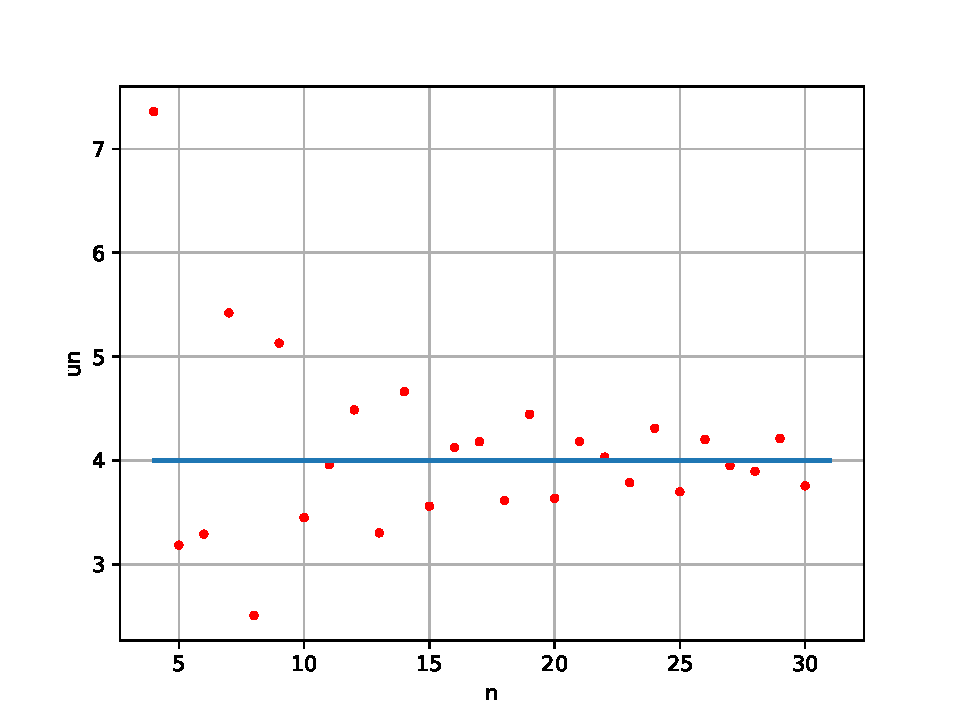
\includegraphics[width=0.85\textwidth]{resources/convergence.pdf}
	\caption{Un exemple de suite convergente.}
\end{figure}

\begin{exer}
Les suites suivantes convergent-elles ?
\begin{multicols}{2}
\begin{itemize}
	\item $u_n = \dfrac1n +1$
	\item $u_n = \sin\left(\dfrac{n\pi}{2}\right) $
	\item $u_n = \dfrac 1n\sin\left(\dfrac 1n\right)$
	\item $u_n = \begin{cases}
	1 & \text{si }\sqrt n\in\NN\\
	0 & \text{sinon}
	\end{cases}$
\end{itemize}
\end{multicols}
\end{exer}

\begin{defn}[Divergence vers l'infini]
Soit $(u_n)$ une suite de nombres réels. On dit que $u$ \emph{tend vers $+\infty$} si pour tout $A\in\RR$, il existe $n_0\in\NN$ tel que
\[
\forall n\geq n_0\quad u_n \geq A
\]
ou, autrement dit, pour toute borne $A$ que l'on peut se fixer, tous les termes de la suite après $n_0$ dépassent $A$.
\end{defn}

\begin{exer}
Écrire une définition tendre vers $-\infty$.
\end{exer}

On remarquera qu'une suite qui tend vers l'infini ne converge pas.

\begin{exer}
Les suites suivantes tendent-elles vers $\pm\infty$ ?
\begin{itemize}
	\item $u_n = n\frac\pi 2$
	\item $u_n = n\sin\left(n\frac\pi2\right)$
	\item $u_n = n\left(2+\sin\left(n\dfrac\pi2\right)\right)$
\end{itemize}
\end{exer}

\begin{defn}
	Une suite $(u_n)$ est dite \emph{bornée} s'il existe un réel $B > 0$ tel que
	\[
	\forall n\in\NN\quad |u_n|\leq B
	\]
\end{defn}

\begin{prop}
Soient $u$ et $v$ deux suites de nombres réels. On suppose que $u$ est bornée et que $v$ tend vers 0. Alors:
\[
u_nv_n \xrightarrow[n\to\infty]{}0.
\]
\end{prop}

\begin{exer}[Formes indéterminées]
On se propose d'étudier la convergence de suites définies par des fractions dont les numérateurs et dénominateurs divergent.

Tout d'abord,
\[
\dfrac{5n^2 + 4n - 5}{3n^2+2n}
\]

Ensuite,
\[
\frac{5\sqrt n + 4}{6n + 2\sqrt n}\]

\end{exer}

\begin{exer}[Une approximation de la racine carrée de 2]
	On considère la suite de nombres réels $(u_n)$ de premier terme un entier $u_0\geq 2$, vérifiant la relation de récurrence \[
	u_{n+1} = \frac{u_n^2+2}{2u_n}.
	\]
	
	Le but de l'exercice est de montrer que cette suite constitue une approximation de $\sqrt{2}$.
	\begin{enumerate}
		\item Montrer que $(u_n)$ est une suite de nombres rationnels.\\
		\textbf{Indication} On montrera que les termes de la suite s'écrivent $u_n = p_n/q_n$ où $(p_n)$ et $(q_n)$ sont des suites de nombres entiers.
		\item Montrer que pour tout $n$, $u_n \geq \sqrt 2$.
		\item En étudiant le signe de $u_{n+1} - u_n$, montrer que $(u_n)$ est décroissante.
		\item Conclure.
	\end{enumerate}
\end{exer}

\subsection*{Suites de nombres complexes}

Vous connaissez déjà la notion de suite de nombres réels. On définit ci-après la notion de suite de nombres complexes:
\begin{defn}[Suite complexe]
Une \textit{suite de nombres complexes} est une application de l'ensemble $\NN$ des entiers naturels dans l'ensemble $\CC$ des nombres complexes. Étant donné une suite $u$, on appelle \textit{terme} les images $u(n)$ des entiers $n$ par $u$, et on les note plutôt $u_n$. La suite $u$ se note alors classiquement $(u_n)_{n\in\NN}$.
\end{defn}

\begin{exem}
La suite définie par $u_n = (2+i)^n$ est une suite de nombres complexes. Il en est de même de la suite $\left((1/2)^n\right)$ (en effet, toute suite de nombres réels est aussi une suite de nombres complexes puisque $\RR\subset \CC$).
\end{exem}

Pour analyser le comportement d'une suite de réels, vous avez défini en cours les notions de \textit{convergence} et de \textit{limite}. La définition suivante étend alors le concept à une suite de complexes.

\begin{defn}
Soit $(z_n)_{n\in\NN}$ une suite de nombres complexes. Soit $\ell \in\CC$. On dit que \textit{la suite $(z_n)$ converge vers $\ell$} lorsque la suite de nombres réels
$\left(
|z_n -\ell|\right)_{n\in\NN}
$
converge vers zéro. On notera comme dans le cas réel
\[
\lim_{n\to\infty}z_n = \ell \quad\text{ou}\quad z_n \xrightarrow[n\to\infty]{}\ell.
\]
\end{defn}

\begin{exer}
Soit $(z_n)$ une suite de nombres complexes.\begin{enumerate}
	\item Montrer qu'il existe deux suites de nombres réels $(a_n)_{n\in\NN}$ et $(b_n)_{n\in\NN}$ telles que
	\[
	\forall n\in\NN \quad z_n = a_n + ib_n.
	\]
	\item Montrer que si $(z_n)$ converge vers une limite $\ell\in\CC$, alors les suites $(a_n)$ et $(b_n)$ également, et exprimer leurs limites.
	\item Montrer réciproquement que si les suites $(a_n)$ et $(b_n)$ convergent vers des réels $a$ et $b$, alors $(z_n)$ converge vers une limite qu'on exprimera.
\end{enumerate} 
\noindent\textbf{Indication} On remarquera l'inégalité suivante (démonstration ?):
\[
\forall z\in\CC \quad |\Re(z)| \leq |z|\text{ et }|\Im(z)| \leq |z|
\]
\end{exer}

\begin{exer}
Cet exercice s'intéresse aux conditions de convergence et de périodicité de suites complexes définies par une relation de récurrence simple.
\begin{enumerate}
	\item Soient $a\in\CC$. Déterminer une condition suffisante sur $a$ pour que la suite de relation de récurrence
	\[
	\left\{
	\begin{array}{rll}
	z_{n+1} &= &az_n\\
	z_0 &\in &\CC
	\end{array}
	\right.
	\]
	converge.
	\item Que peut-il se passer si cette condition n'est pas vérifiée ? Distinguer le cas $|a| = 1$.
\end{enumerate}
On dit qu'une suite de complexes $(z_n)_{n\in\NN}$ est \textit{périodique} s'il existe un entier $T\in\NN$ tel que
\[
\forall n\in\NN\quad z_{n+T} = z_n.
\]
On dira alors que $(z_n)$ est \textit{$T$-périodique}. Ainsi, les suites constantes sont périodiques (de toute période), mais ce ne sont pas les seules.
\begin{enumerate}[resume]
	\item On considère encore une suite définie par une relation de récurrence linéaire $z_{n+1} = az_n$. Trouver une condition sur $a$ pour que $(z_n)$ soit périodique et non nulle.
\end{enumerate}

\noindent\textbf{Indication} On montrera qu'alors $|a| = 1$, et on remarquera que les nombres complexes de module 1 s'écrivent sous la forme $a = e^{i\theta}$ où $\theta\in\RR$.
\end{exer}

\begin{figure}[H]
	\centering
	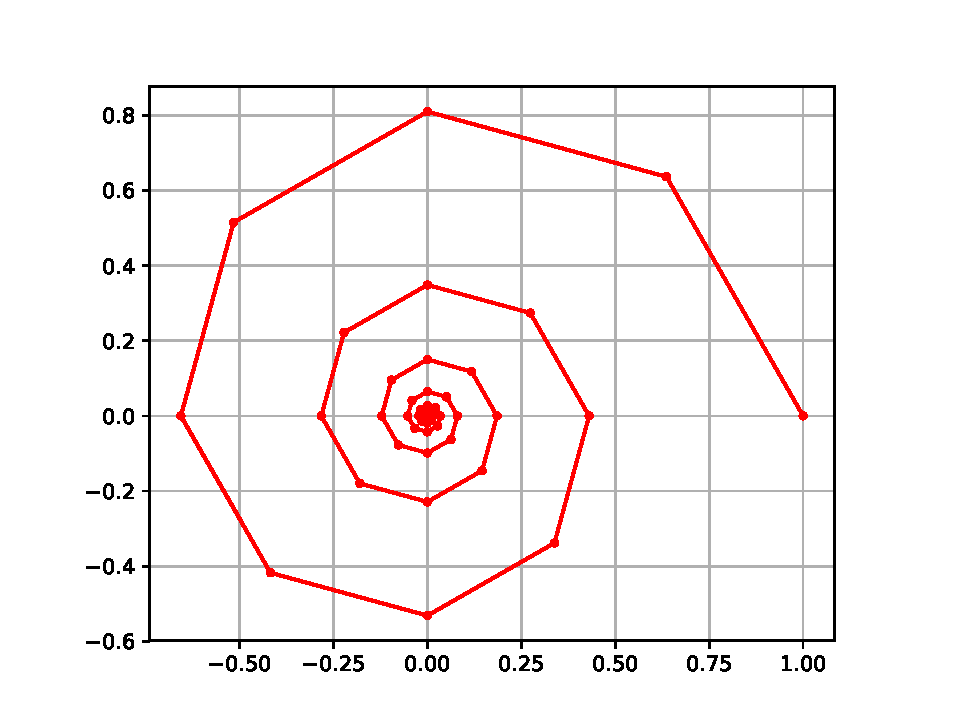
\includegraphics[width=0.86\textwidth]{resources/logaro.pdf}
	\caption{Une spirale logarithmique \textbf{convergente}, avec la relation de récurrence $z_{n+1} = 0,\!9e^{i\pi/4}z_n$. Simulation sous Python avec $N=100$ points.}
\end{figure}

\begin{figure}[H]
	\centering
	\begin{subfigure}{0.84\textwidth}
	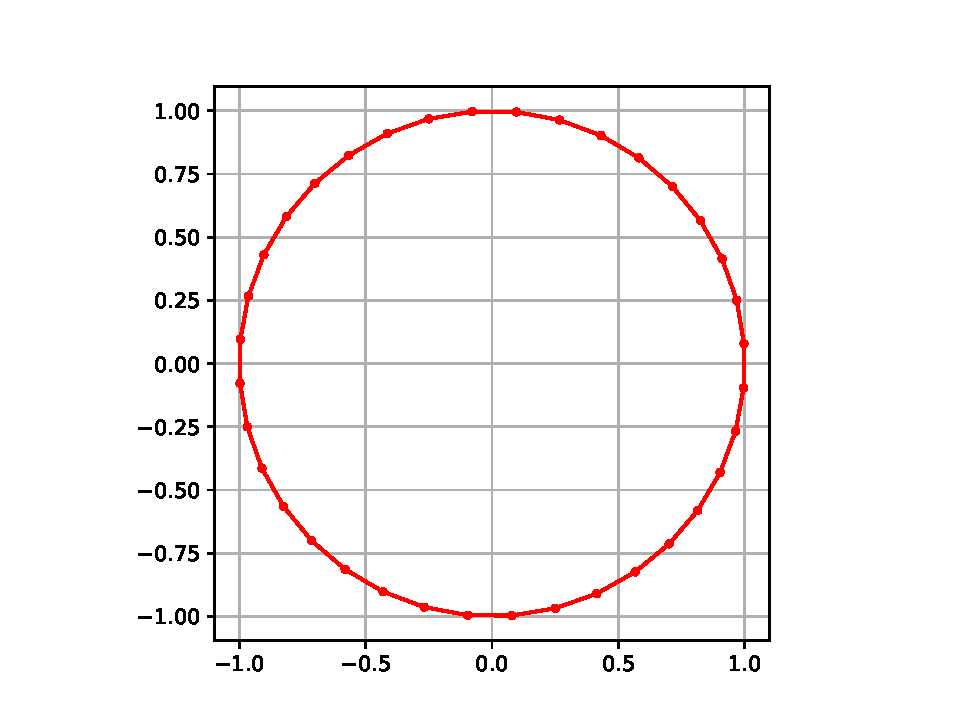
\includegraphics[width=\textwidth]{resources/periodico.pdf}
	\subcaption{Une suite périodique, avec la relation de récurrence $z_{n+1} = e^{i\pi/18}z_n$. $N=36$ points.}
	\end{subfigure}
	
	
	\begin{subfigure}{0.84\textwidth}
	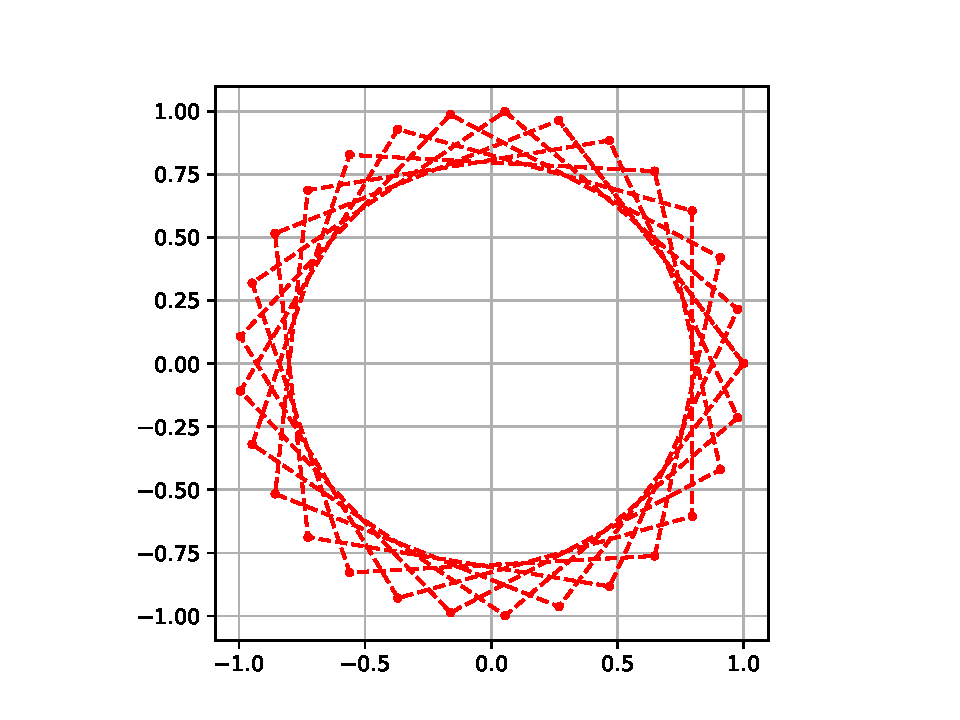
\includegraphics[width=\textwidth]{resources/notperiodico.pdf}
	\subcaption{Un... truc ? avec la relation de récurrence $z_{n+1} = e^{1,3i}z_n$. $N=30$ points.}
	\end{subfigure}
	\caption{Simulations sous Python de suites $z_{n+1} = a^z_n$ avec $|a| = 1$.}
\end{figure}



\begin{figure}[H]
	\centering
	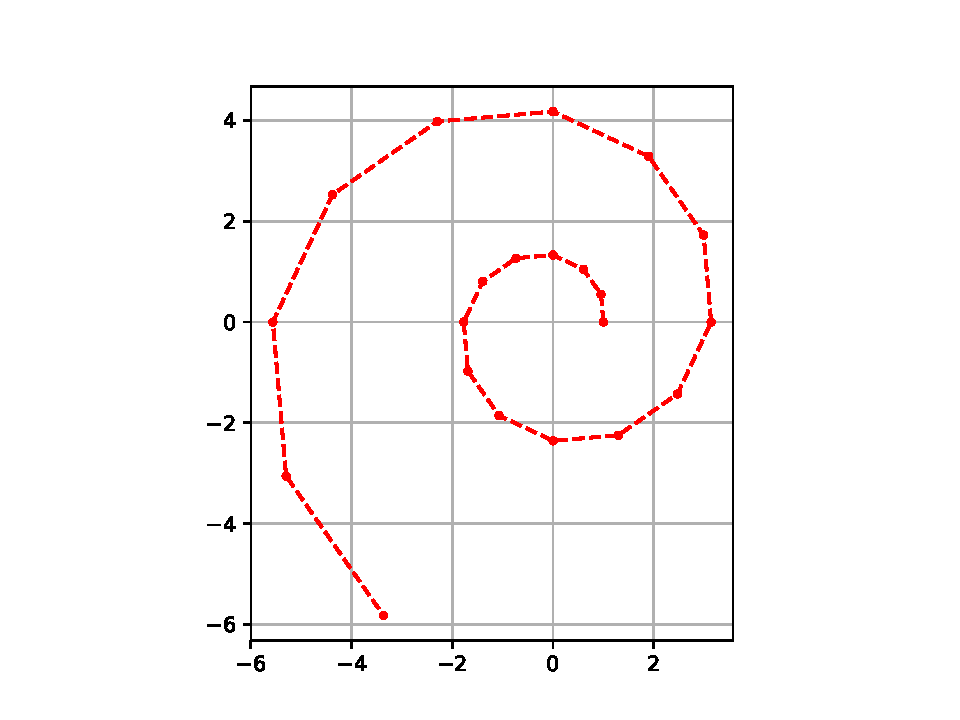
\includegraphics[width=0.86\textwidth]{resources/divergo.pdf}
	\caption{Une spirale logarithmique \textbf{divergente}, avec la relation de récurrence $z_{n+1} = 1,\!1e^{i\pi/6}z_n$. Simulation sous Python avec $N=20$ points.}
\end{figure}

\end{document}